% Appendix D

\chapter{SOWFA Implementation of Feed Forward Derating Control.} % Main appendix title

\label{AppendixD} % For referencing this appendix elsewhere, use \ref{AppendixA}

This appendix documents the controller implementation discussed in Section \ref{section6-2}. The code shown below is a FORTRAN implementation of the Simulink based controller documented in Chapter \ref{Chapter4} and Appendix \ref{sectionB-3} with a few additions.  These subroutines, modules, and code changes are added to the SOWFA/FAST source code, which enables SOWFA to model feed forward derating control. This controller is used for simulations documented in Chapter \ref{Chapter6}.




%----------------------------------------------------------------------------------------
%	SECTION 1
%----------------------------------------------------------------------------------------
\section{Subroutine PitchCtrl()} \label{sectionD-1}
The following subroutine is added to UserSubs.f90:

\noindent
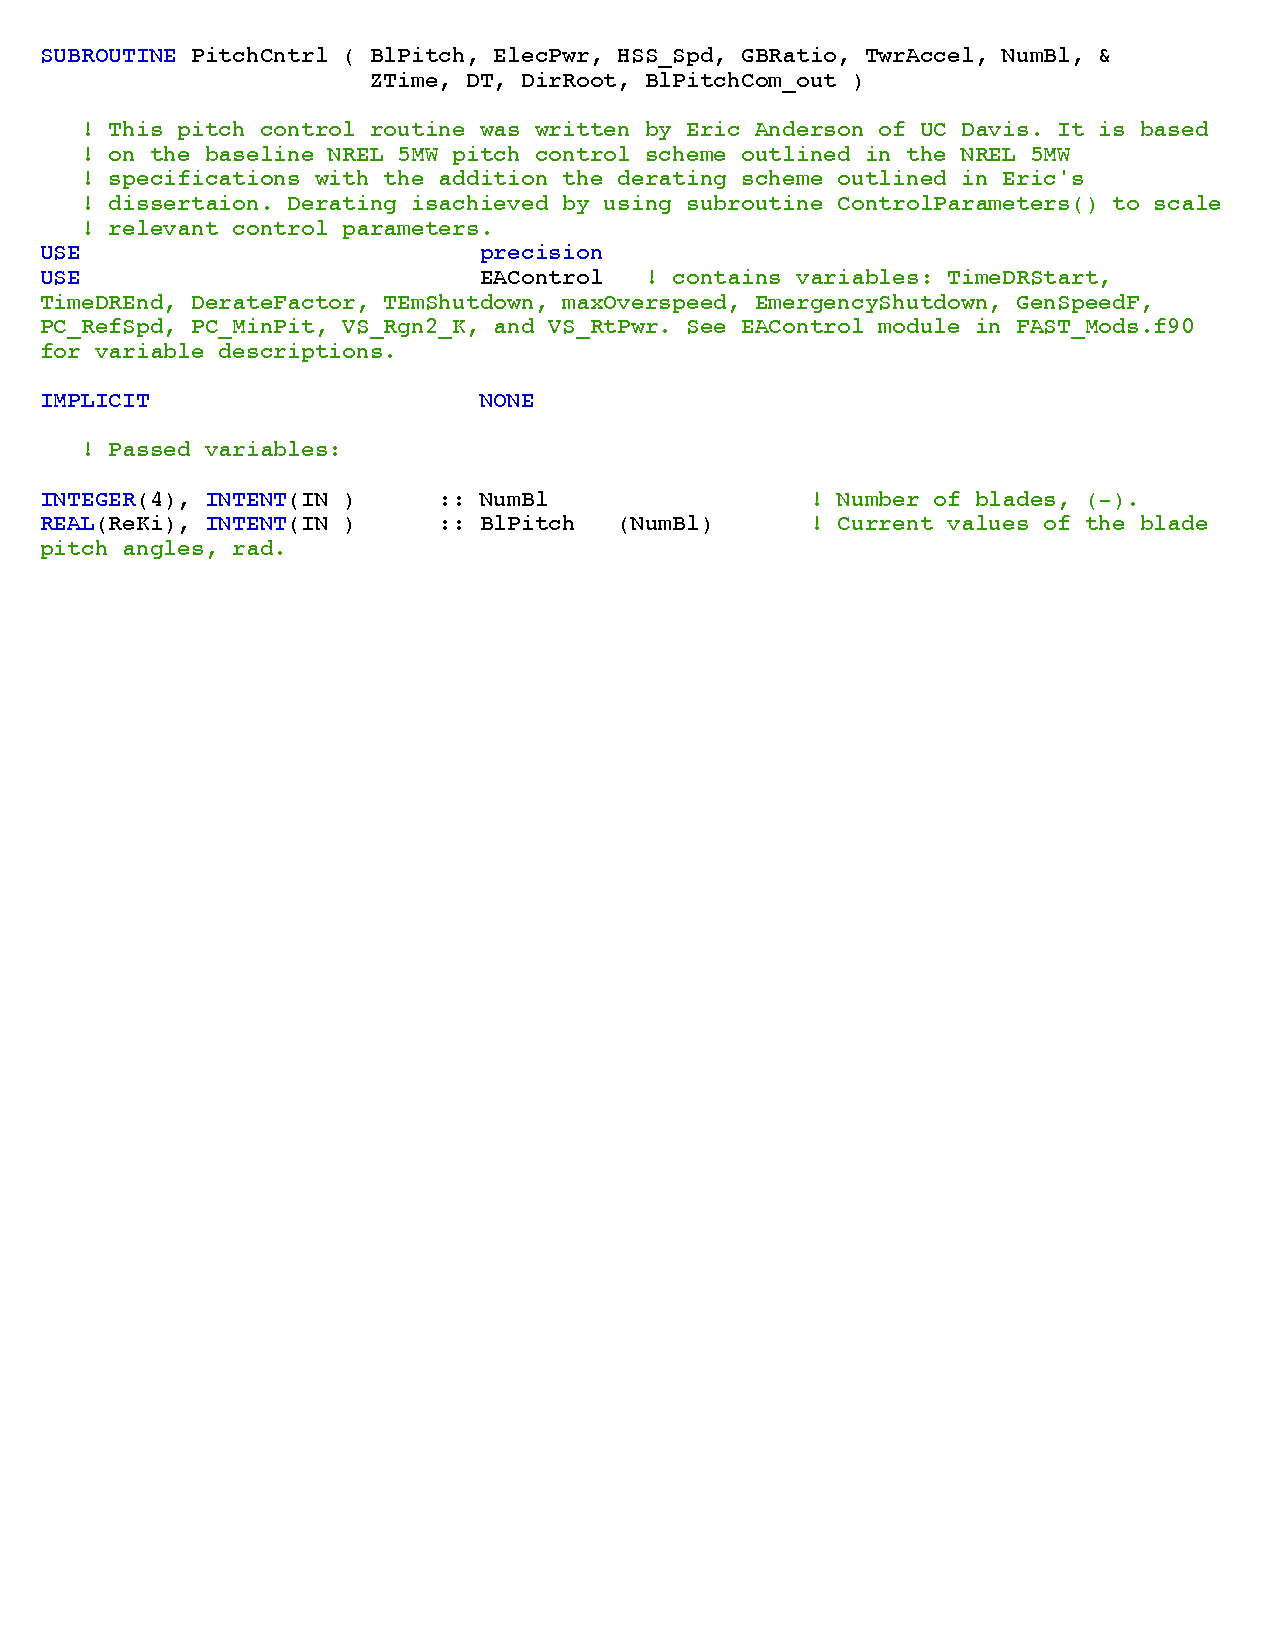
\includegraphics[width=\linewidth]{Figures/AppendixDFigures/figD-1A.pdf}

\noindent
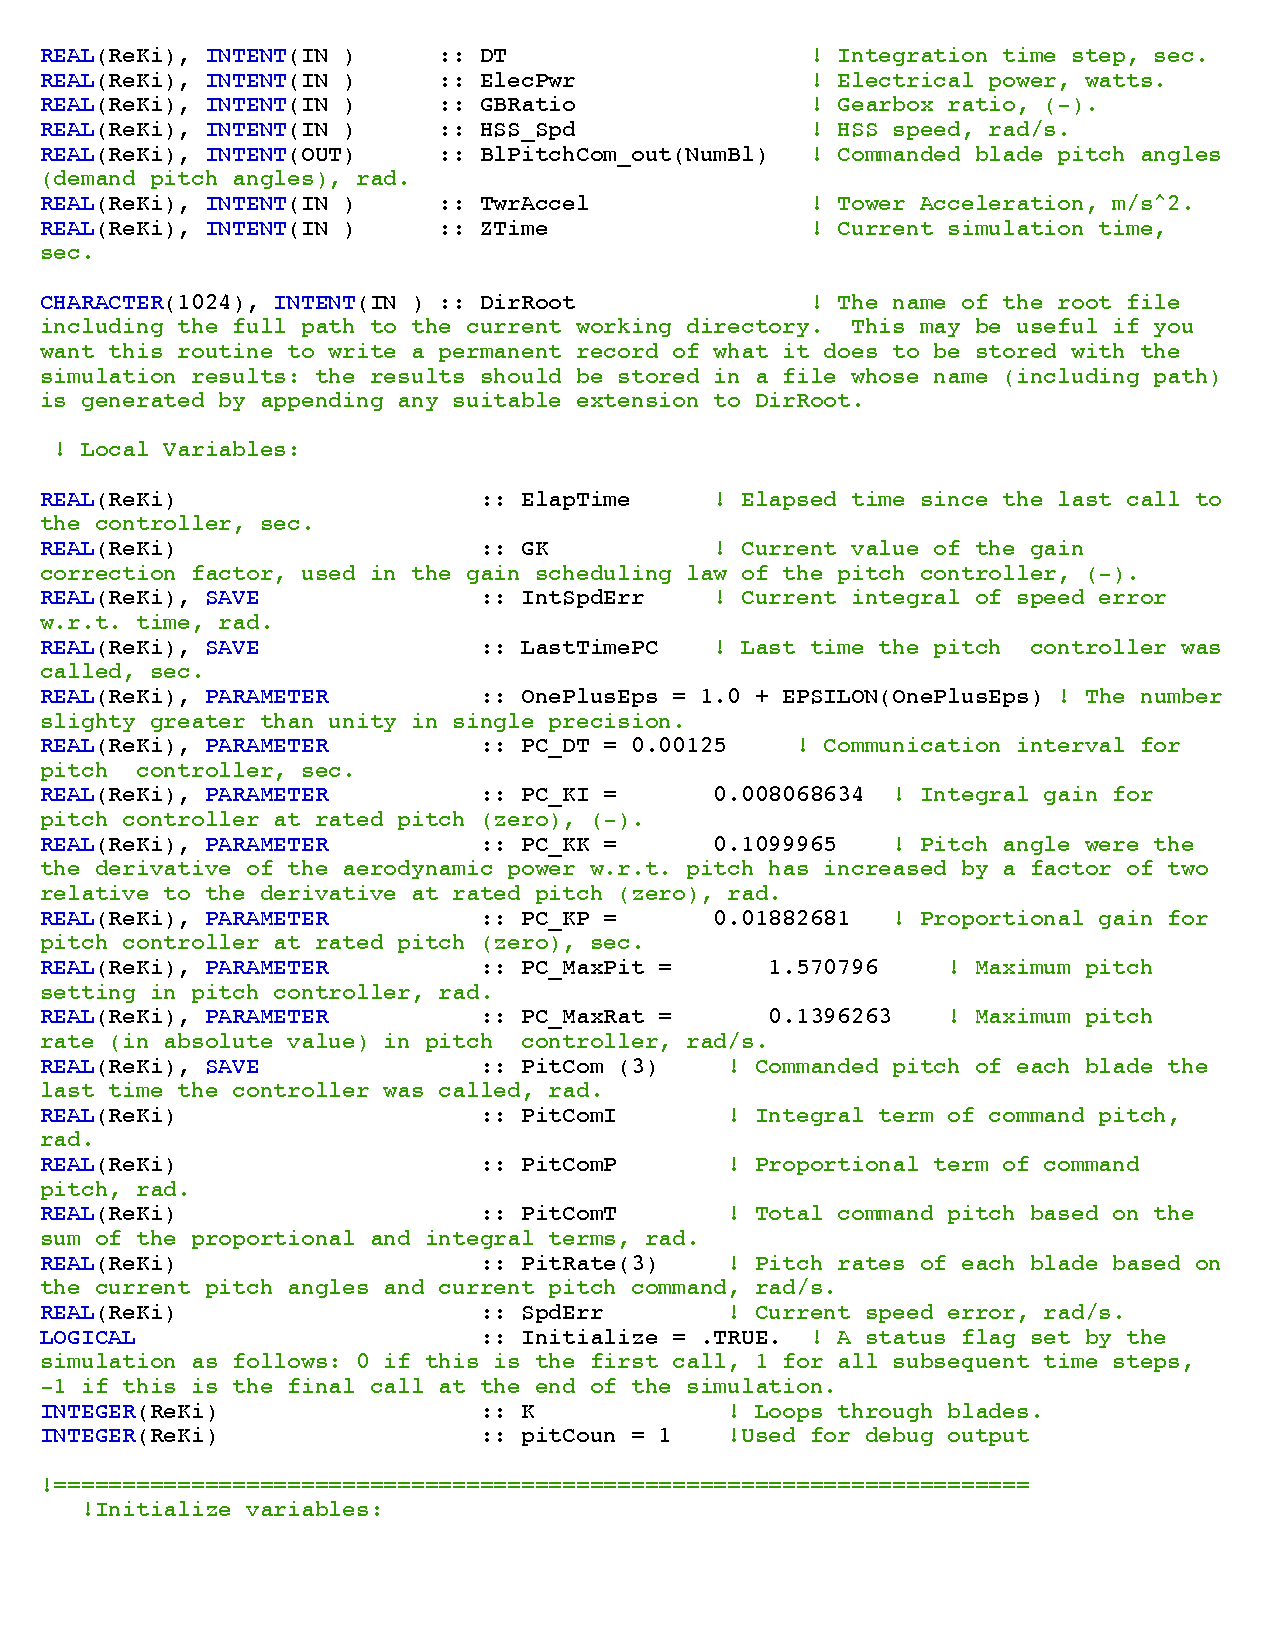
\includegraphics[width=\linewidth]{Figures/AppendixDFigures/figD-1B.pdf}

\noindent
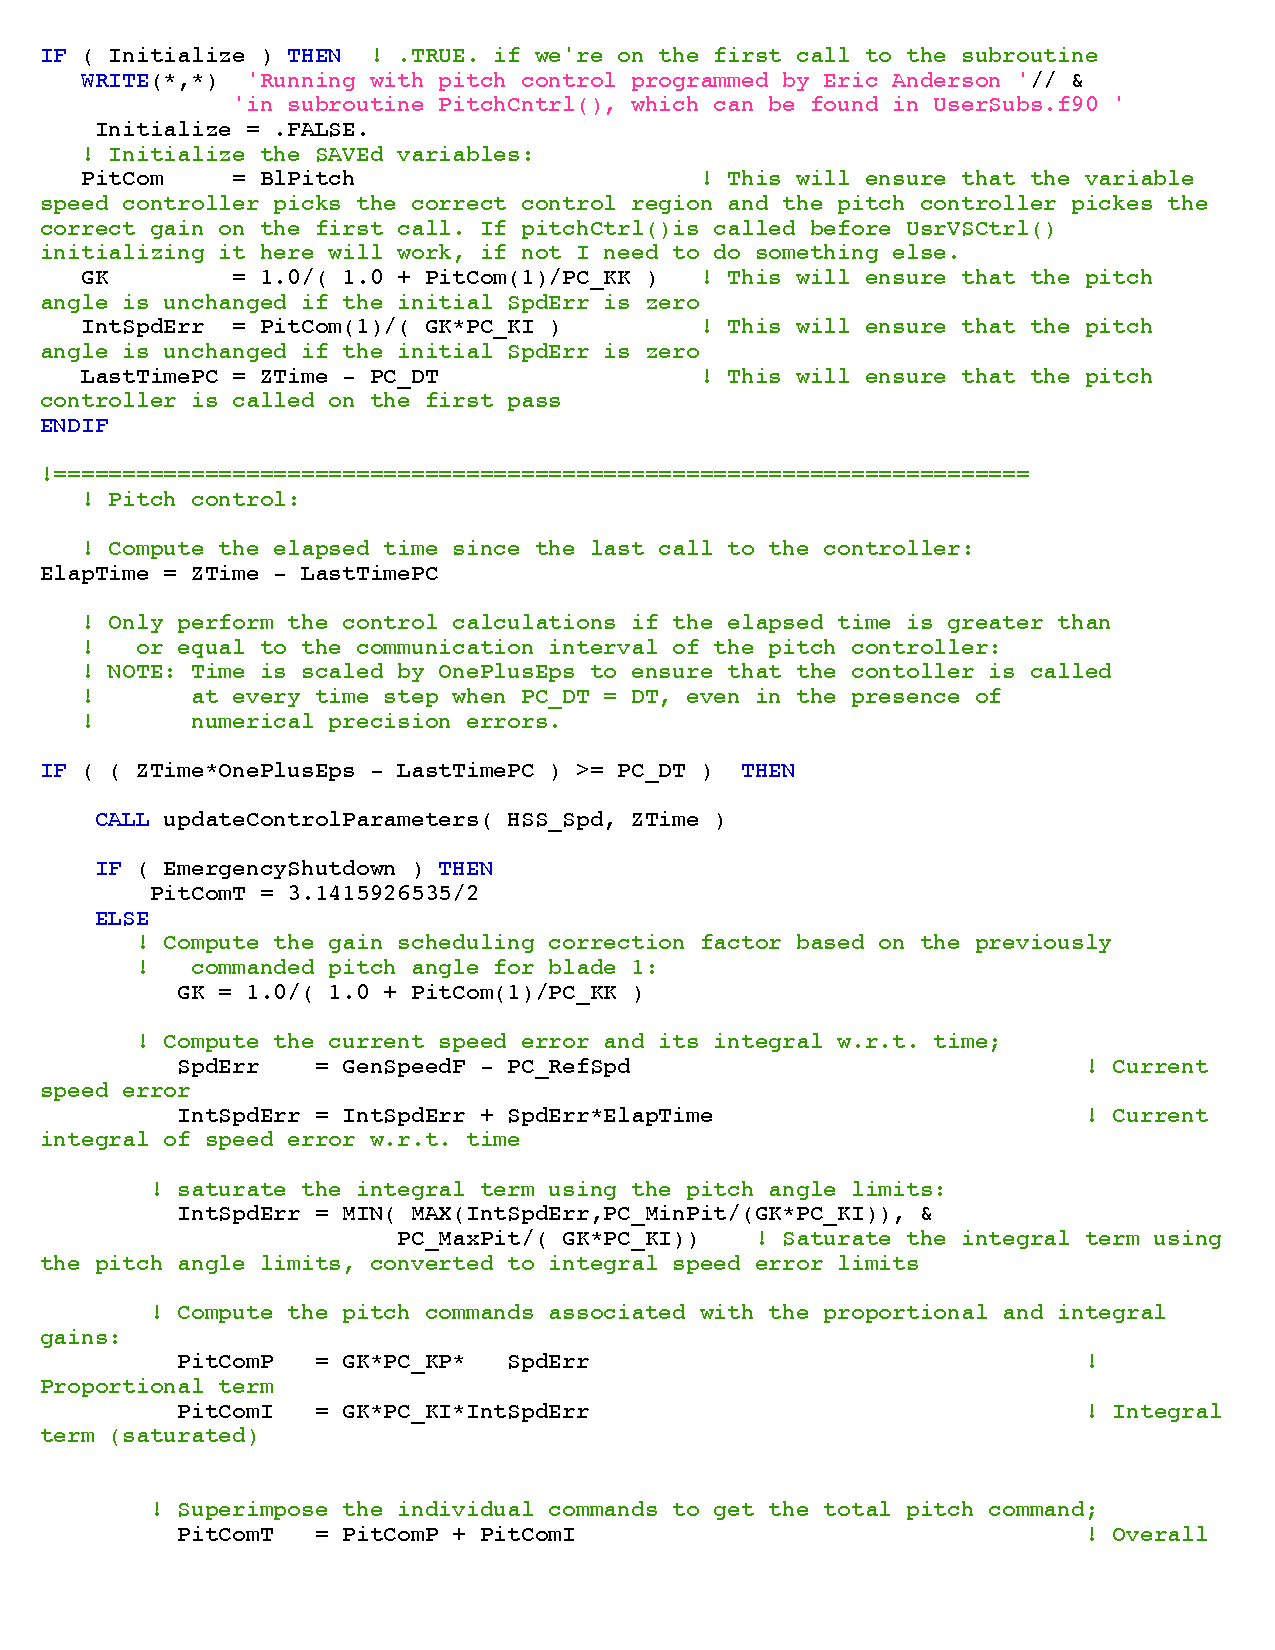
\includegraphics[width=\linewidth]{Figures/AppendixDFigures/figD-1C.pdf}

\noindent
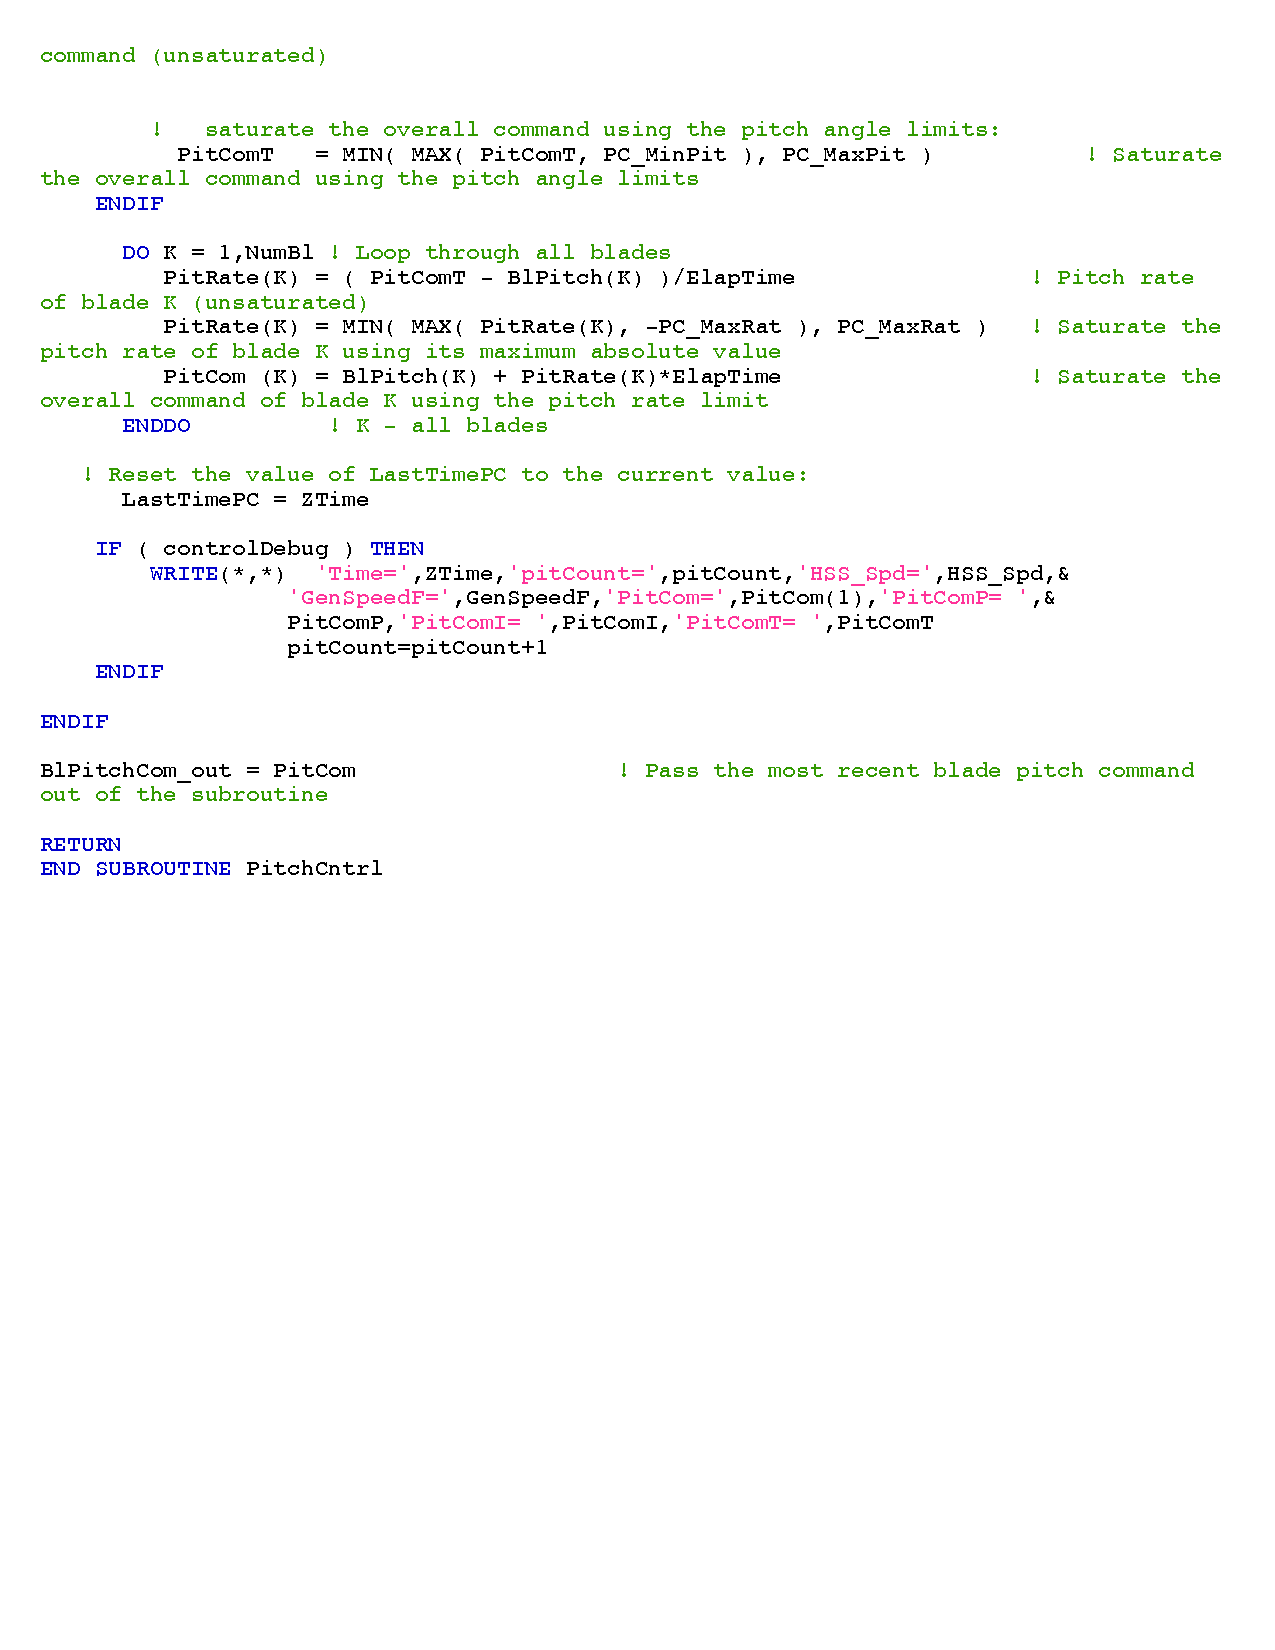
\includegraphics[width=\linewidth]{Figures/AppendixDFigures/figD-1D.pdf}


%----------------------------------------------------------------------------------------
%	SECTION 2
%----------------------------------------------------------------------------------------
\section{Subroutine UserVSCntrl()} \label{sectionD-2}
The following subroutine is added to UserSubs.f90:

\noindent
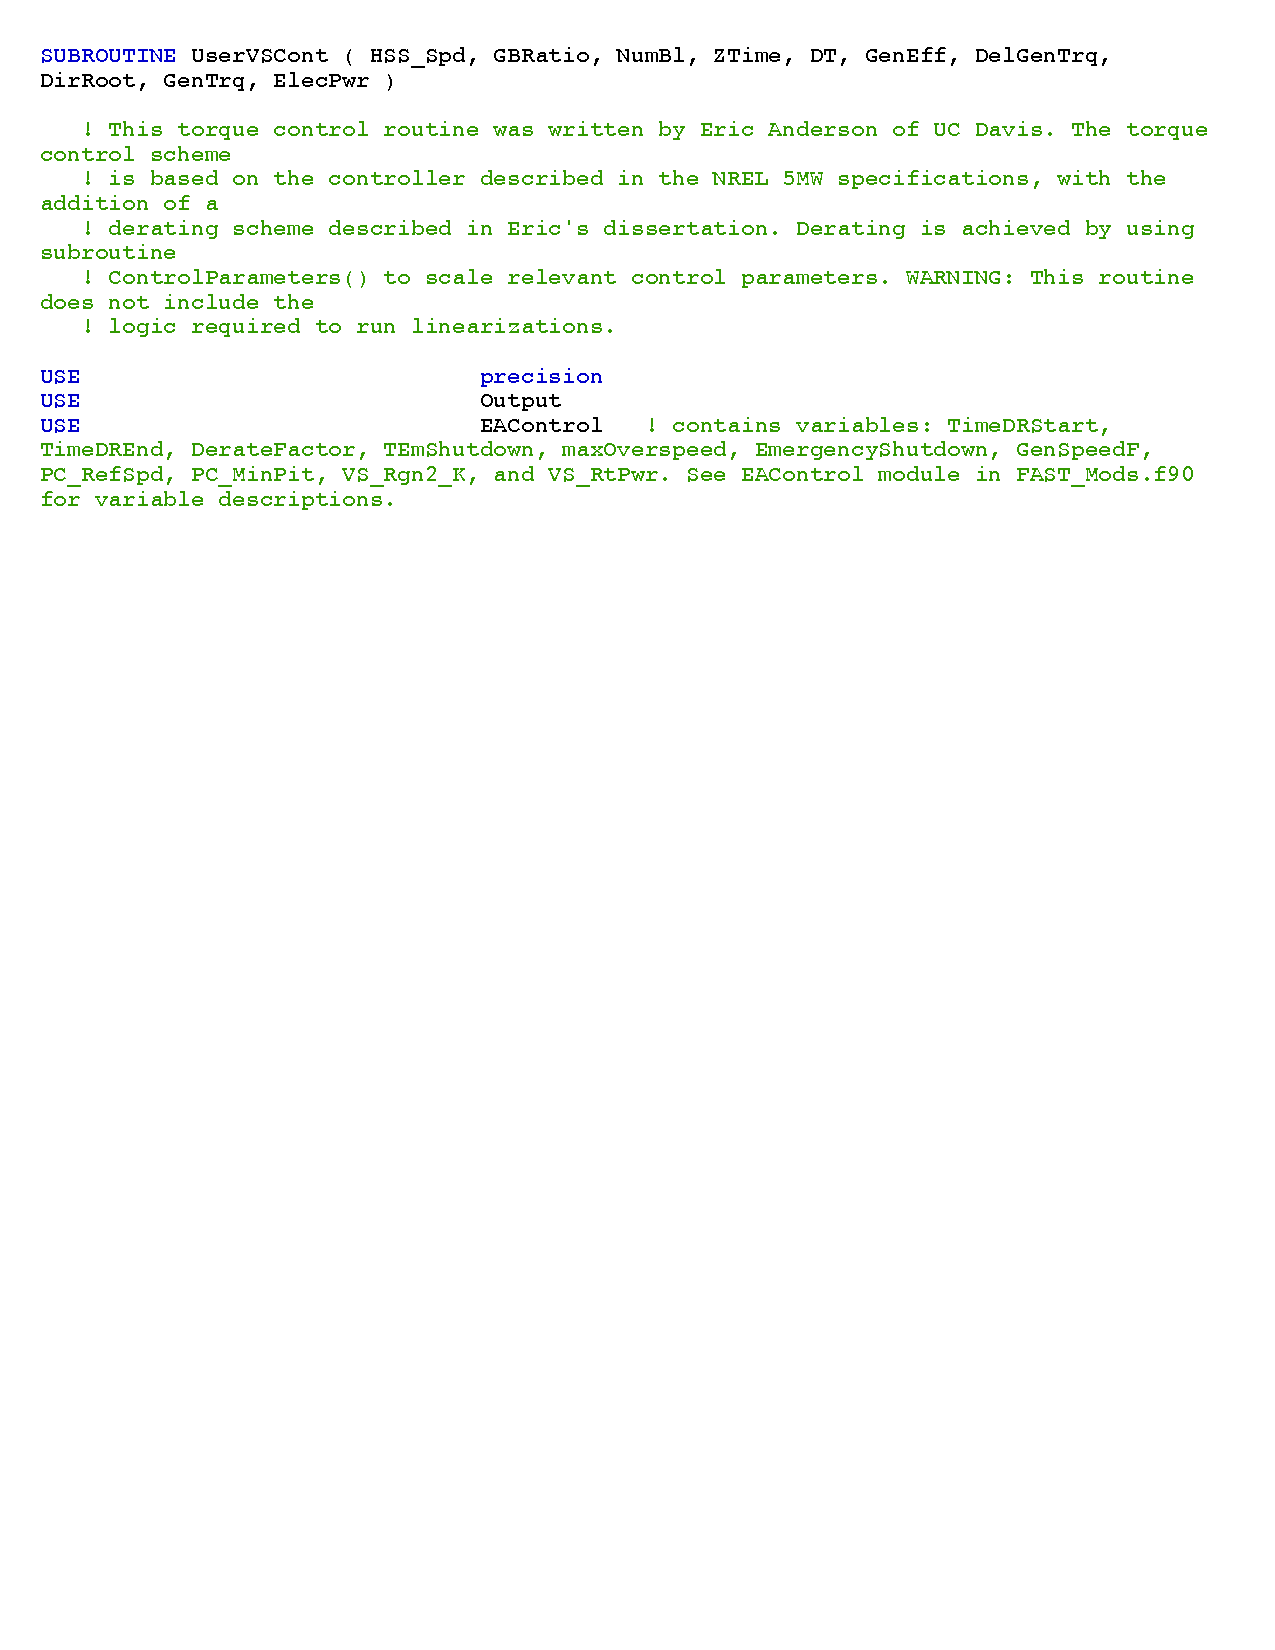
\includegraphics[width=\linewidth]{Figures/AppendixDFigures/figD-2A.pdf}

\noindent
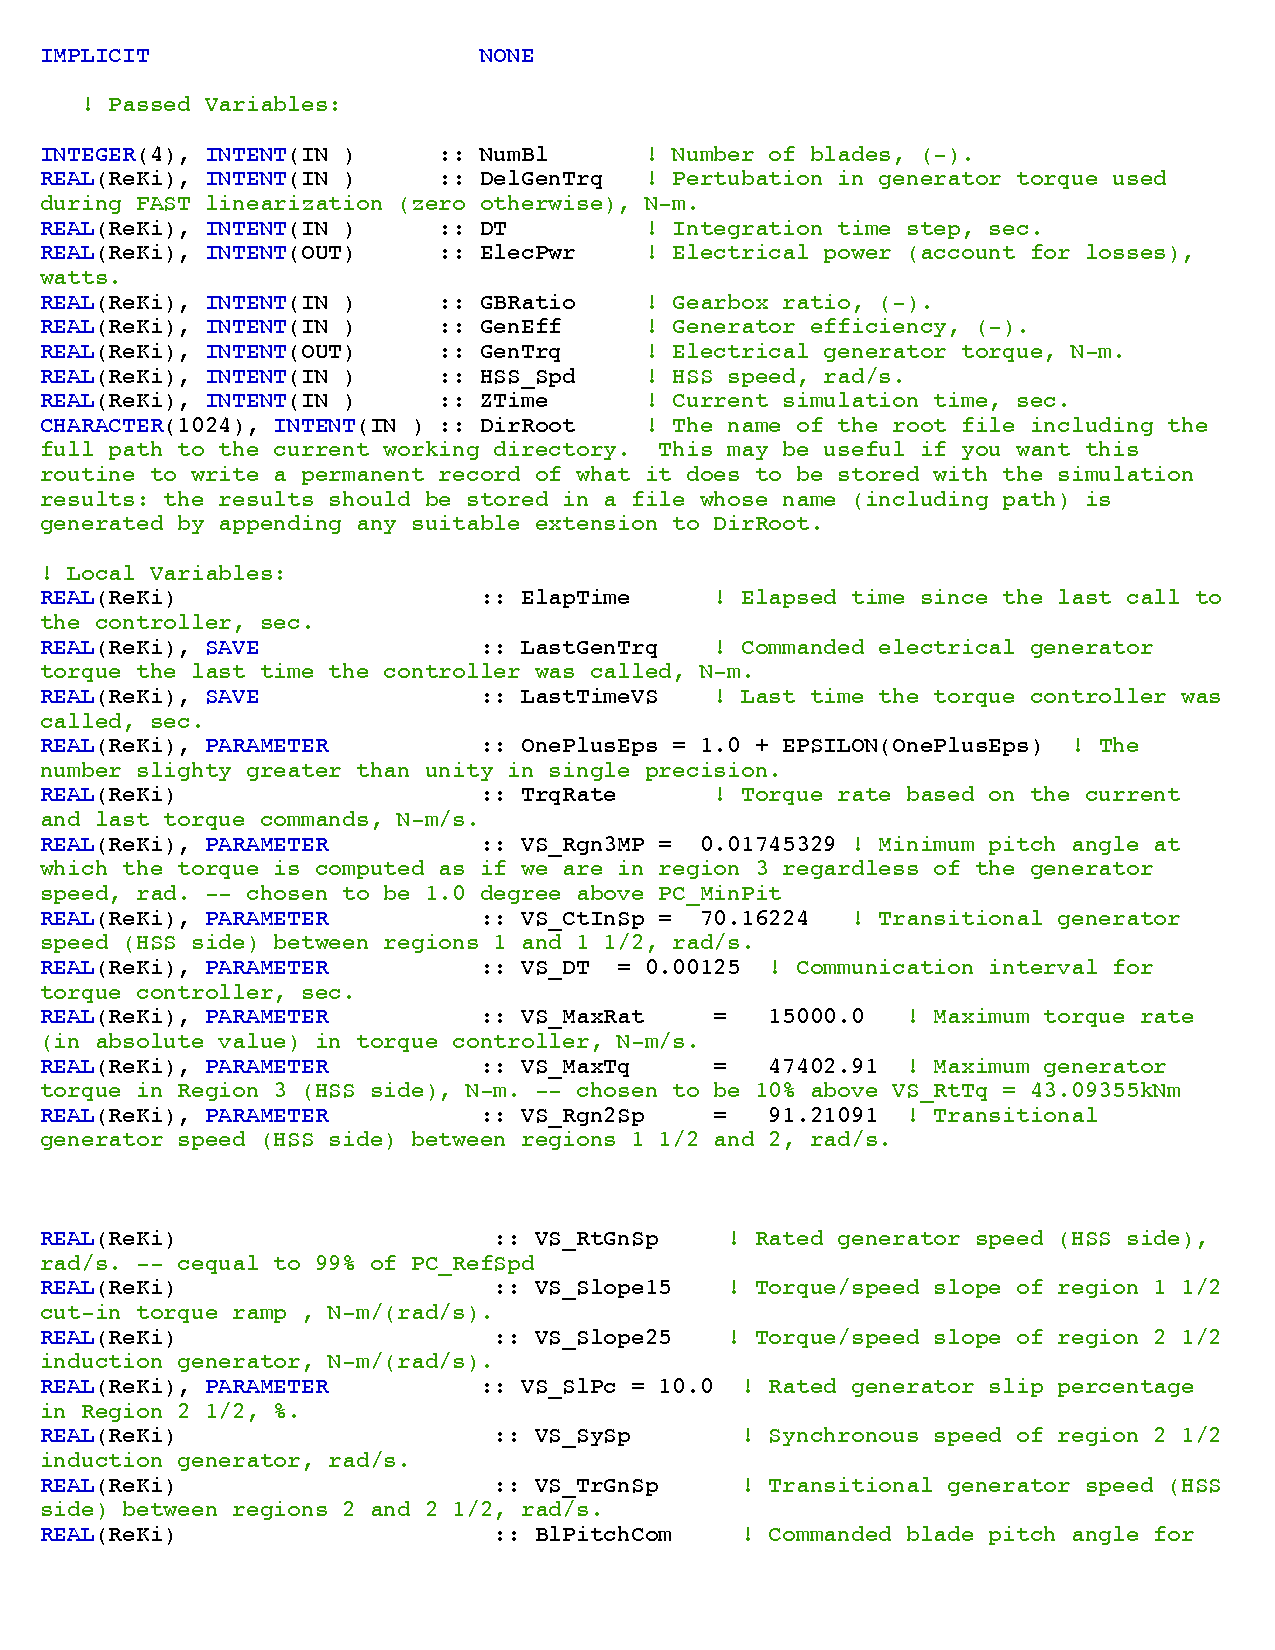
\includegraphics[width=\linewidth]{Figures/AppendixDFigures/figD-2B.pdf}

\noindent
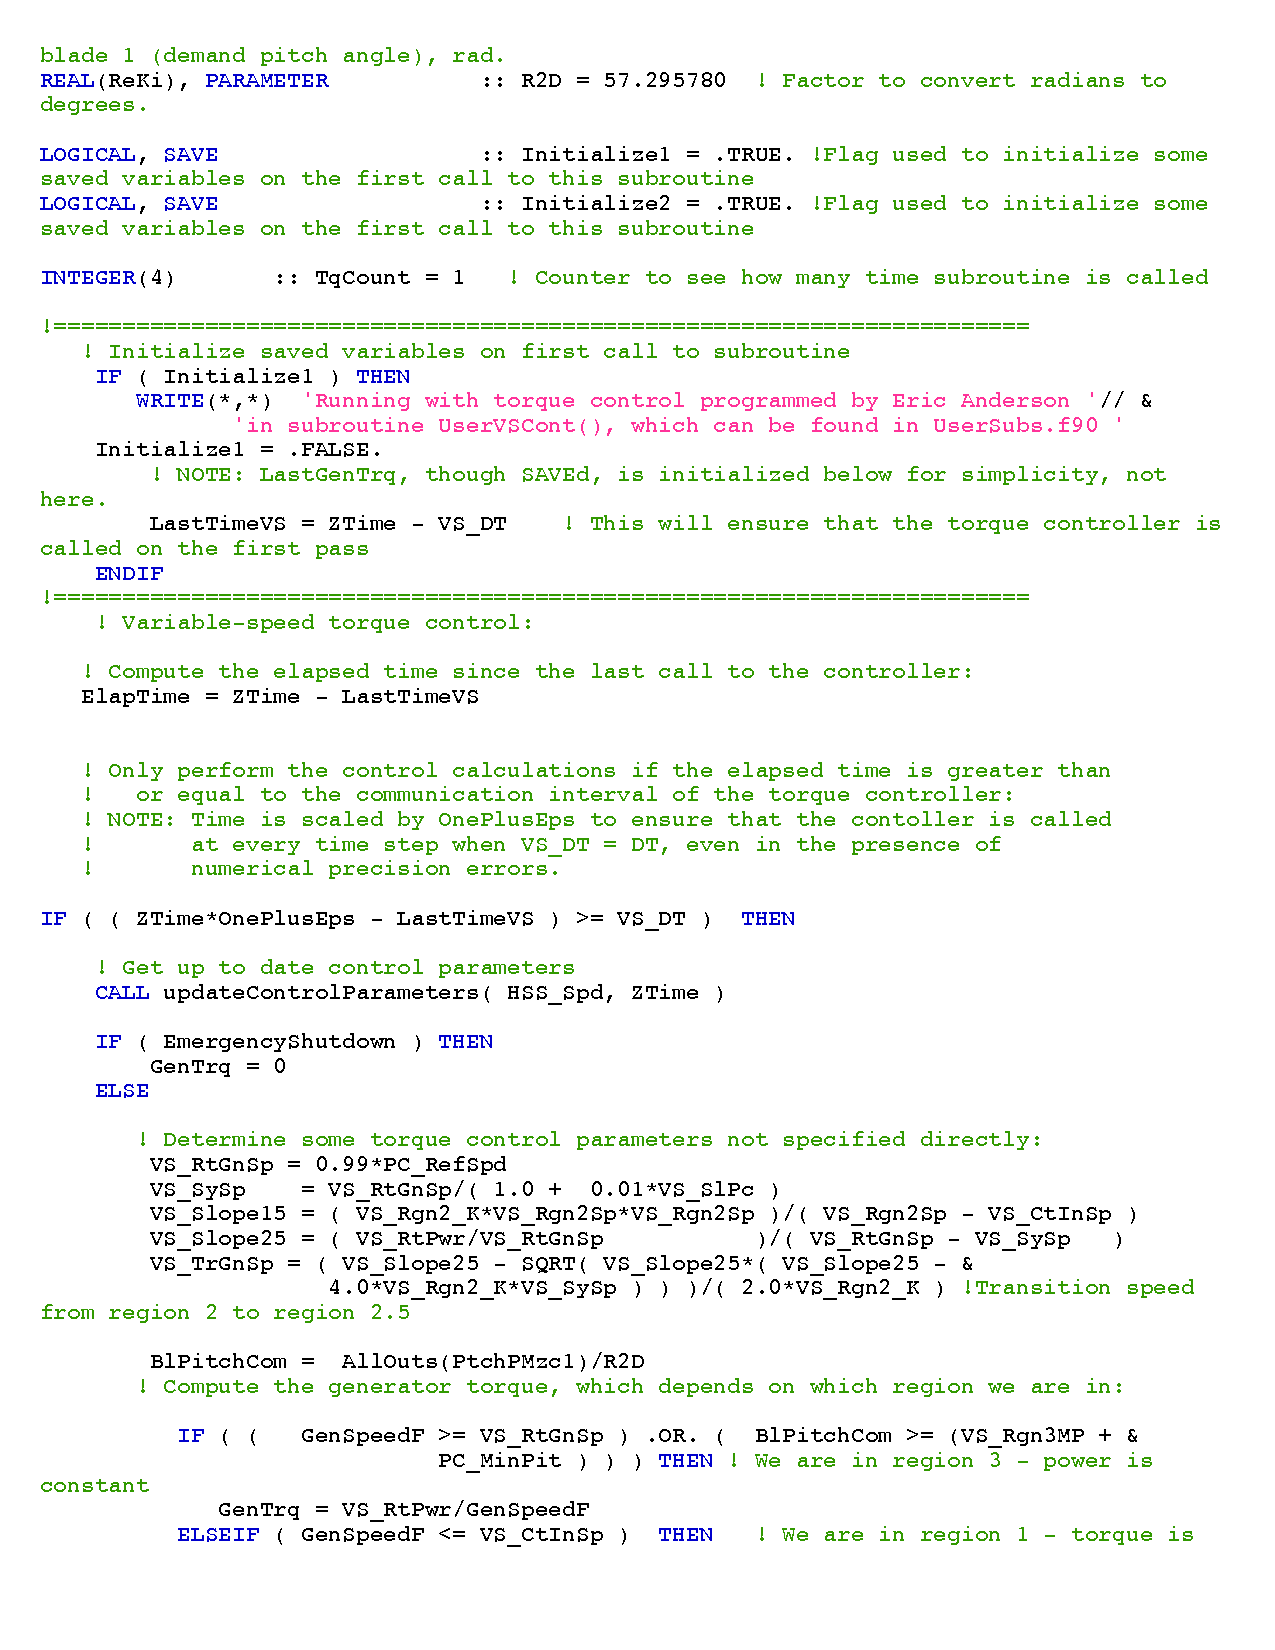
\includegraphics[width=\linewidth]{Figures/AppendixDFigures/figD-2C.pdf}

\noindent
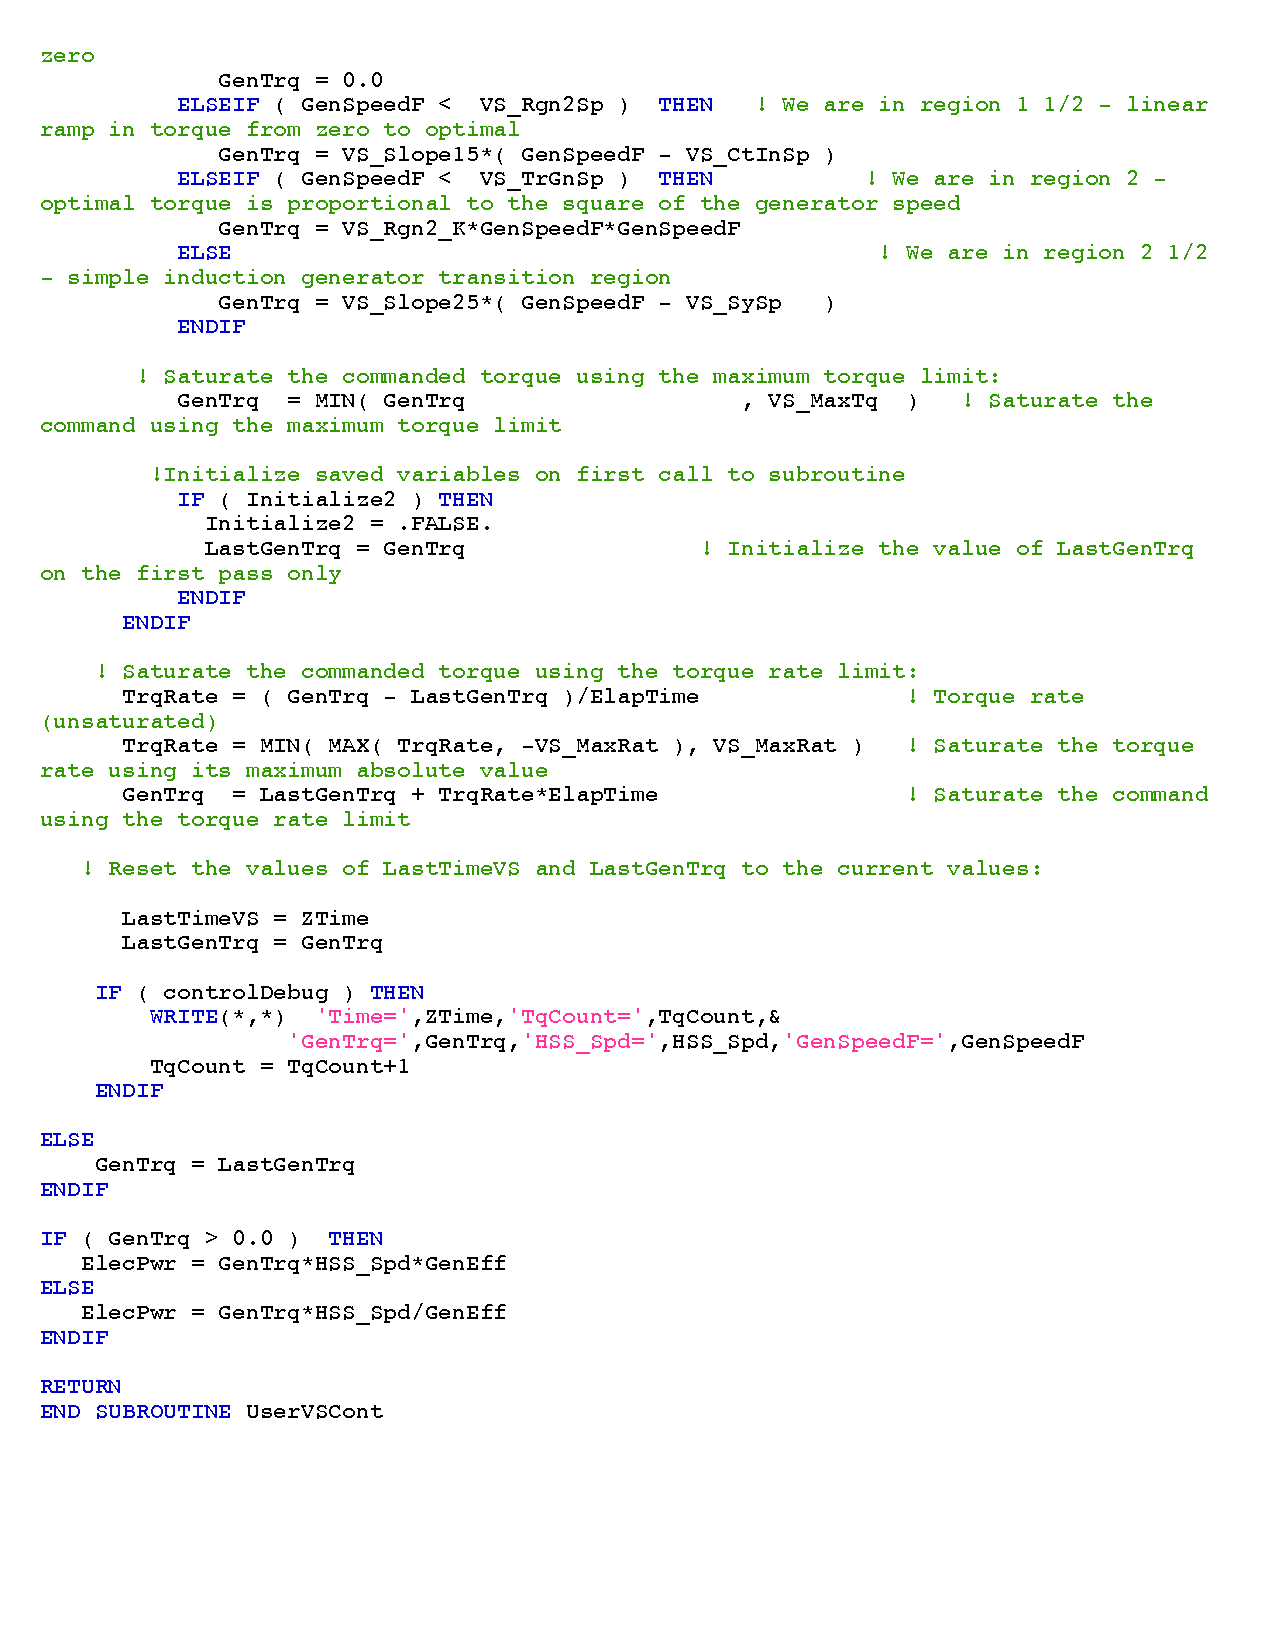
\includegraphics[width=\linewidth]{Figures/AppendixDFigures/figD-2D.pdf}


%----------------------------------------------------------------------------------------
%	SECTION 3
%----------------------------------------------------------------------------------------
\section{Subroutine updateControlParameters()} \label{sectionD-3}
The following subroutine is added to UserSubs.f90.

\noindent
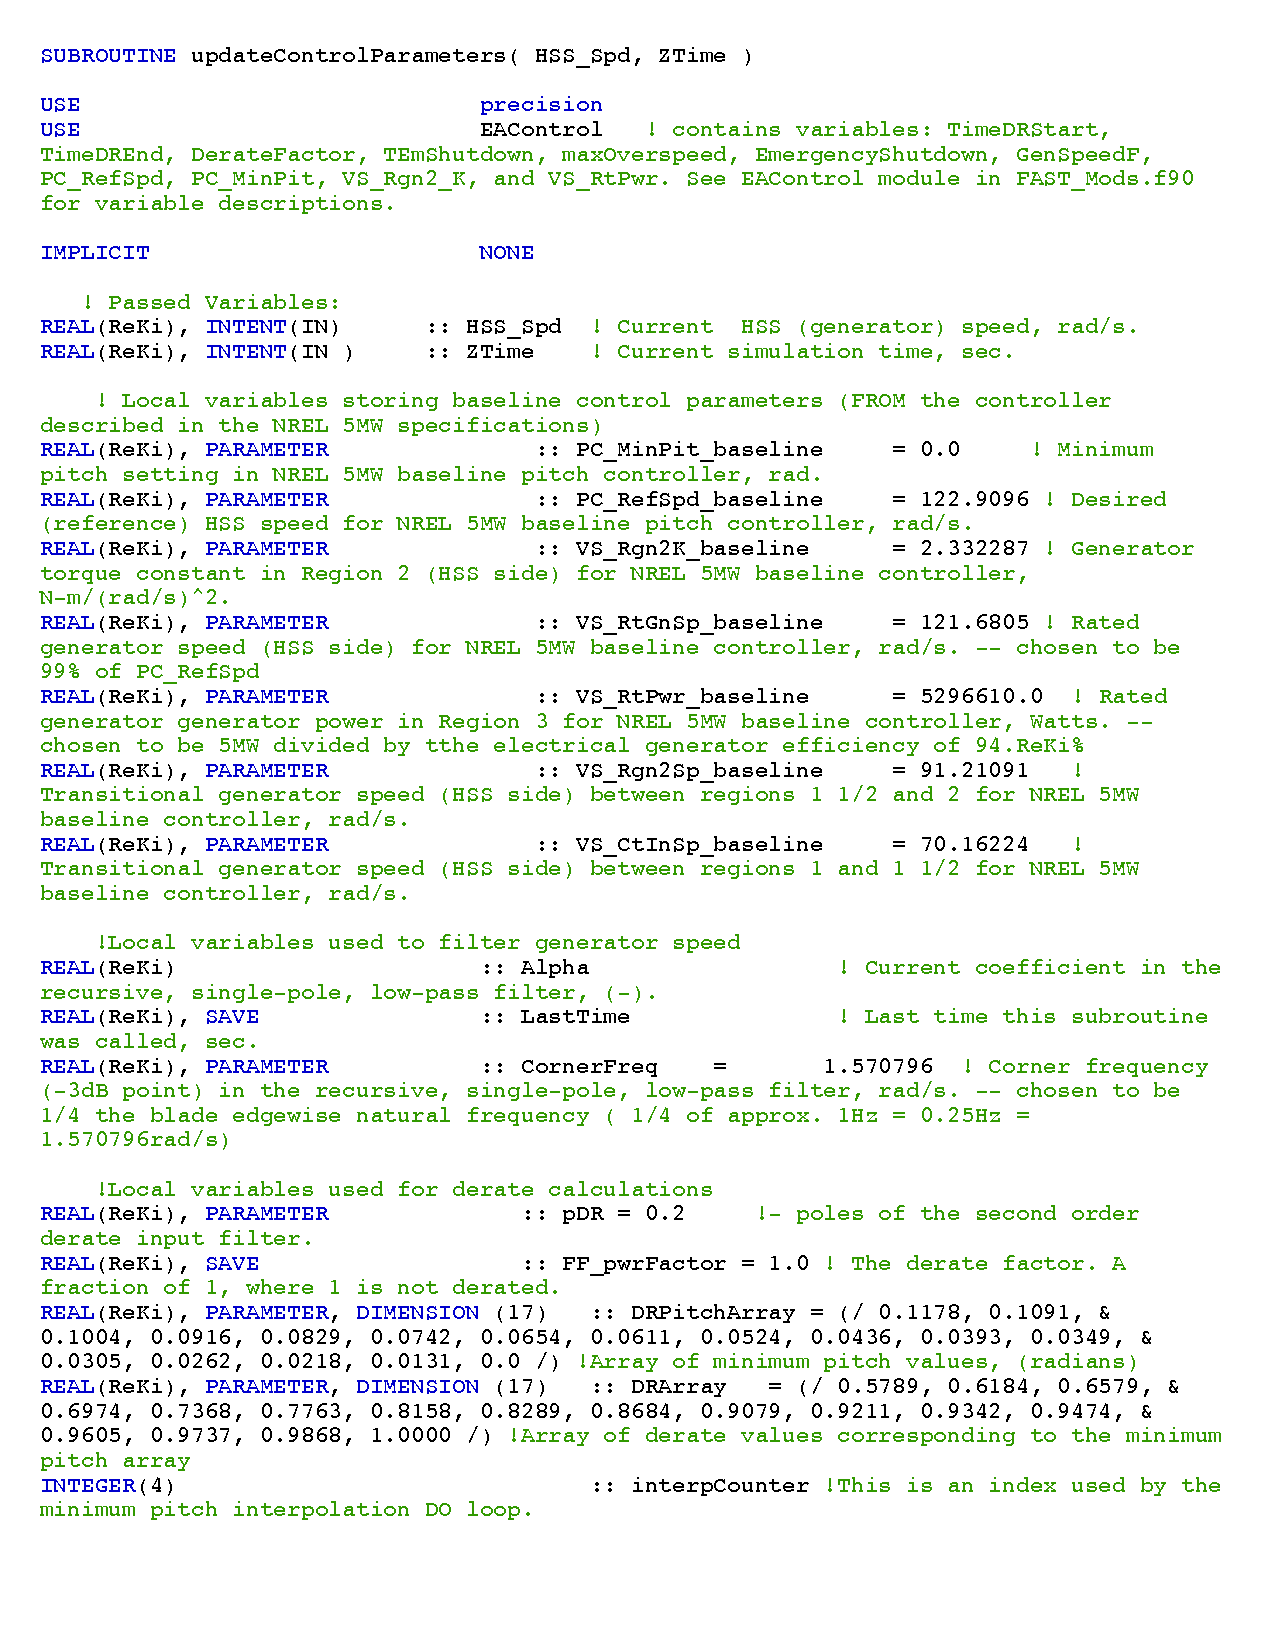
\includegraphics[width=\linewidth]{Figures/AppendixDFigures/figD-3A.pdf}

\noindent
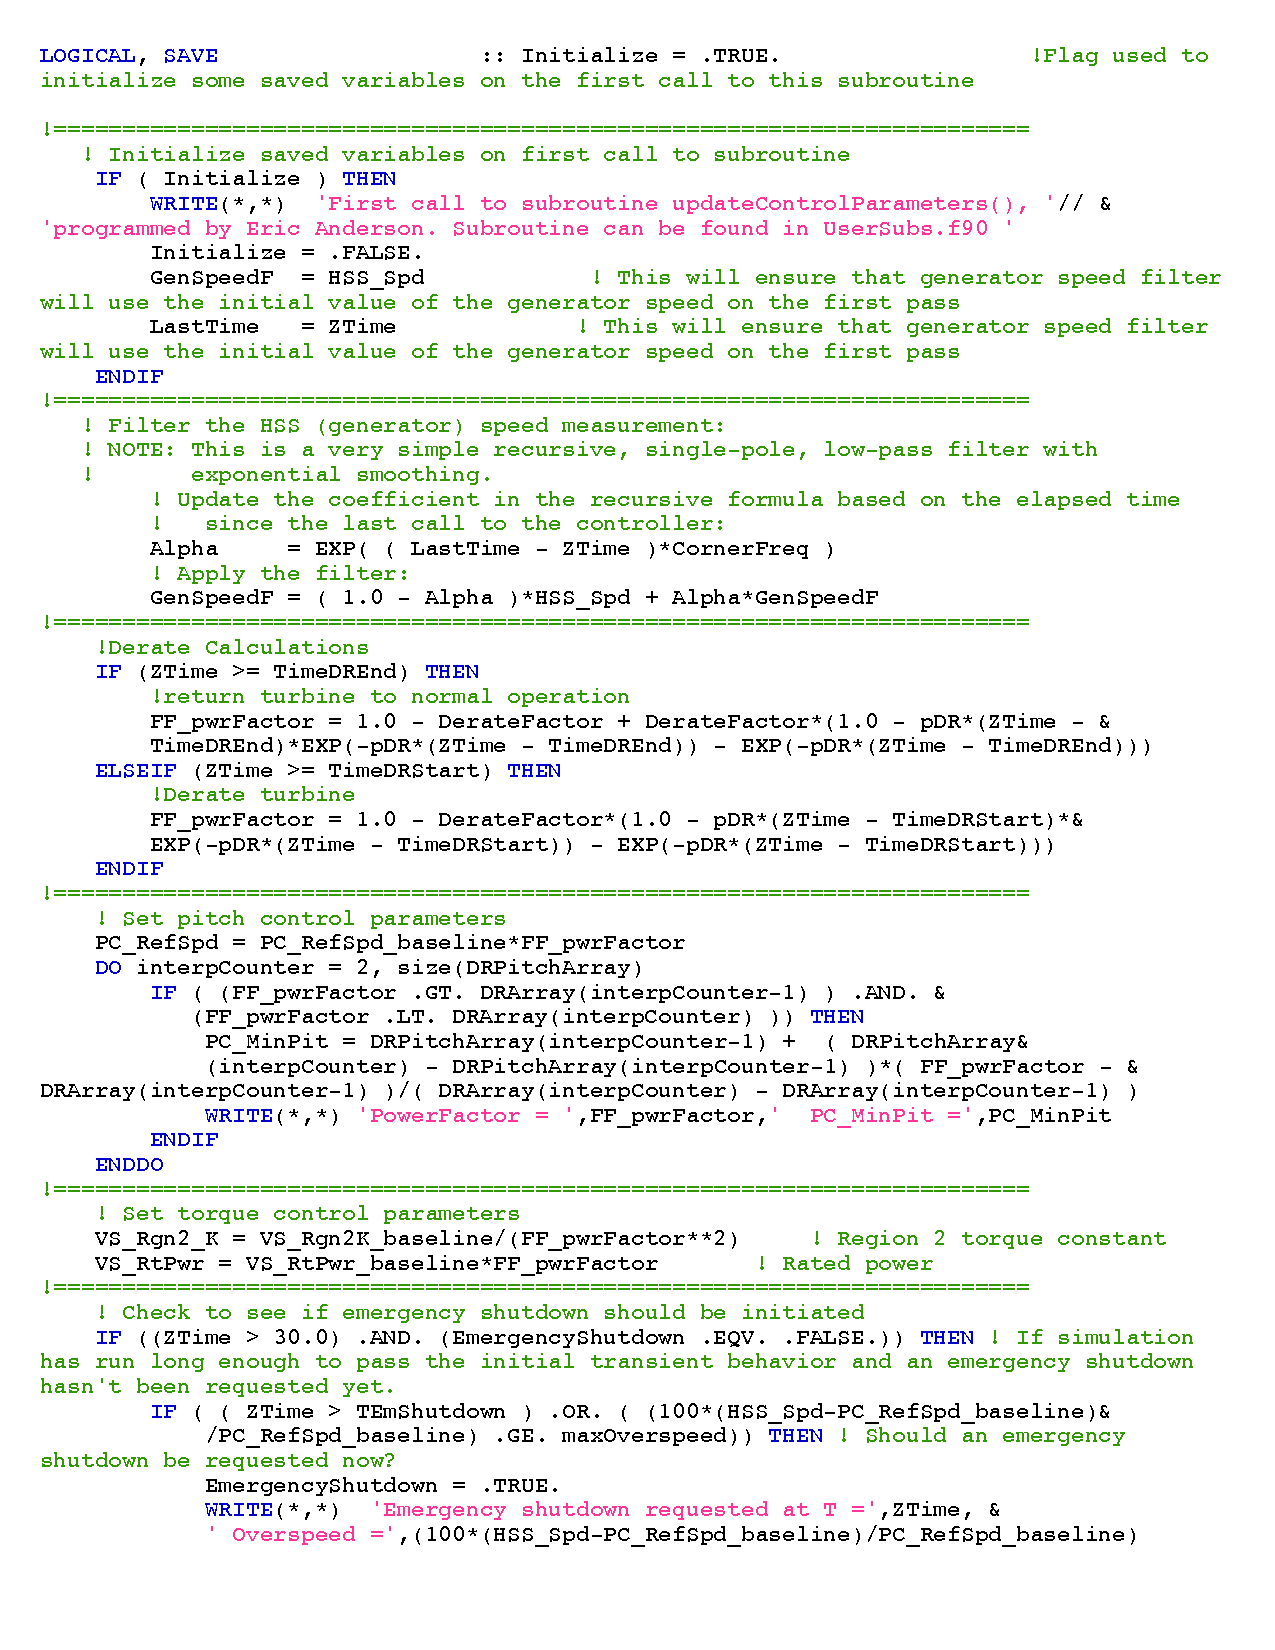
\includegraphics[width=\linewidth]{Figures/AppendixDFigures/figD-3B.pdf}

\noindent
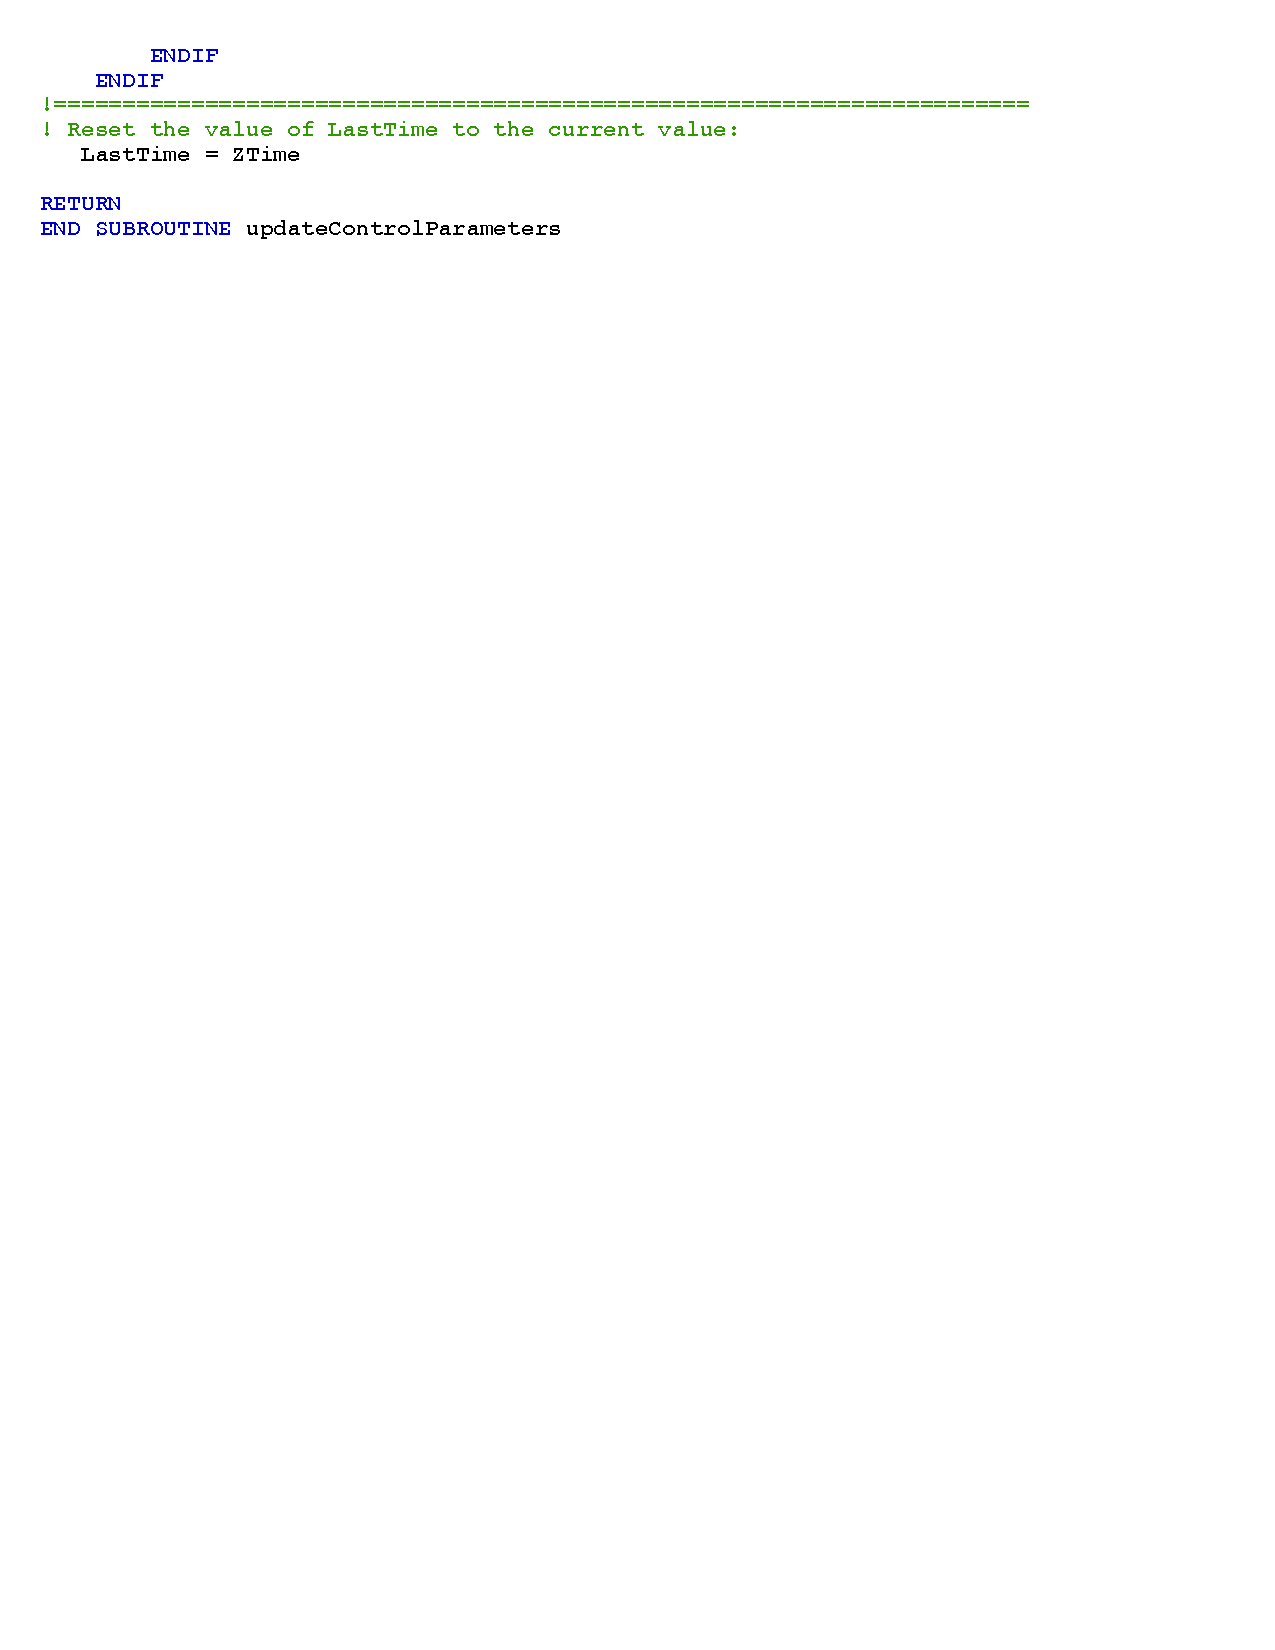
\includegraphics[width=\linewidth]{Figures/AppendixDFigures/figD-3C.pdf}

%----------------------------------------------------------------------------------------
%	SECTION 4
%----------------------------------------------------------------------------------------
\section{Subroutine UserHSSBr()} \label{sectionD-4}
The following subroutine is added to UserSubs.f90.

\noindent
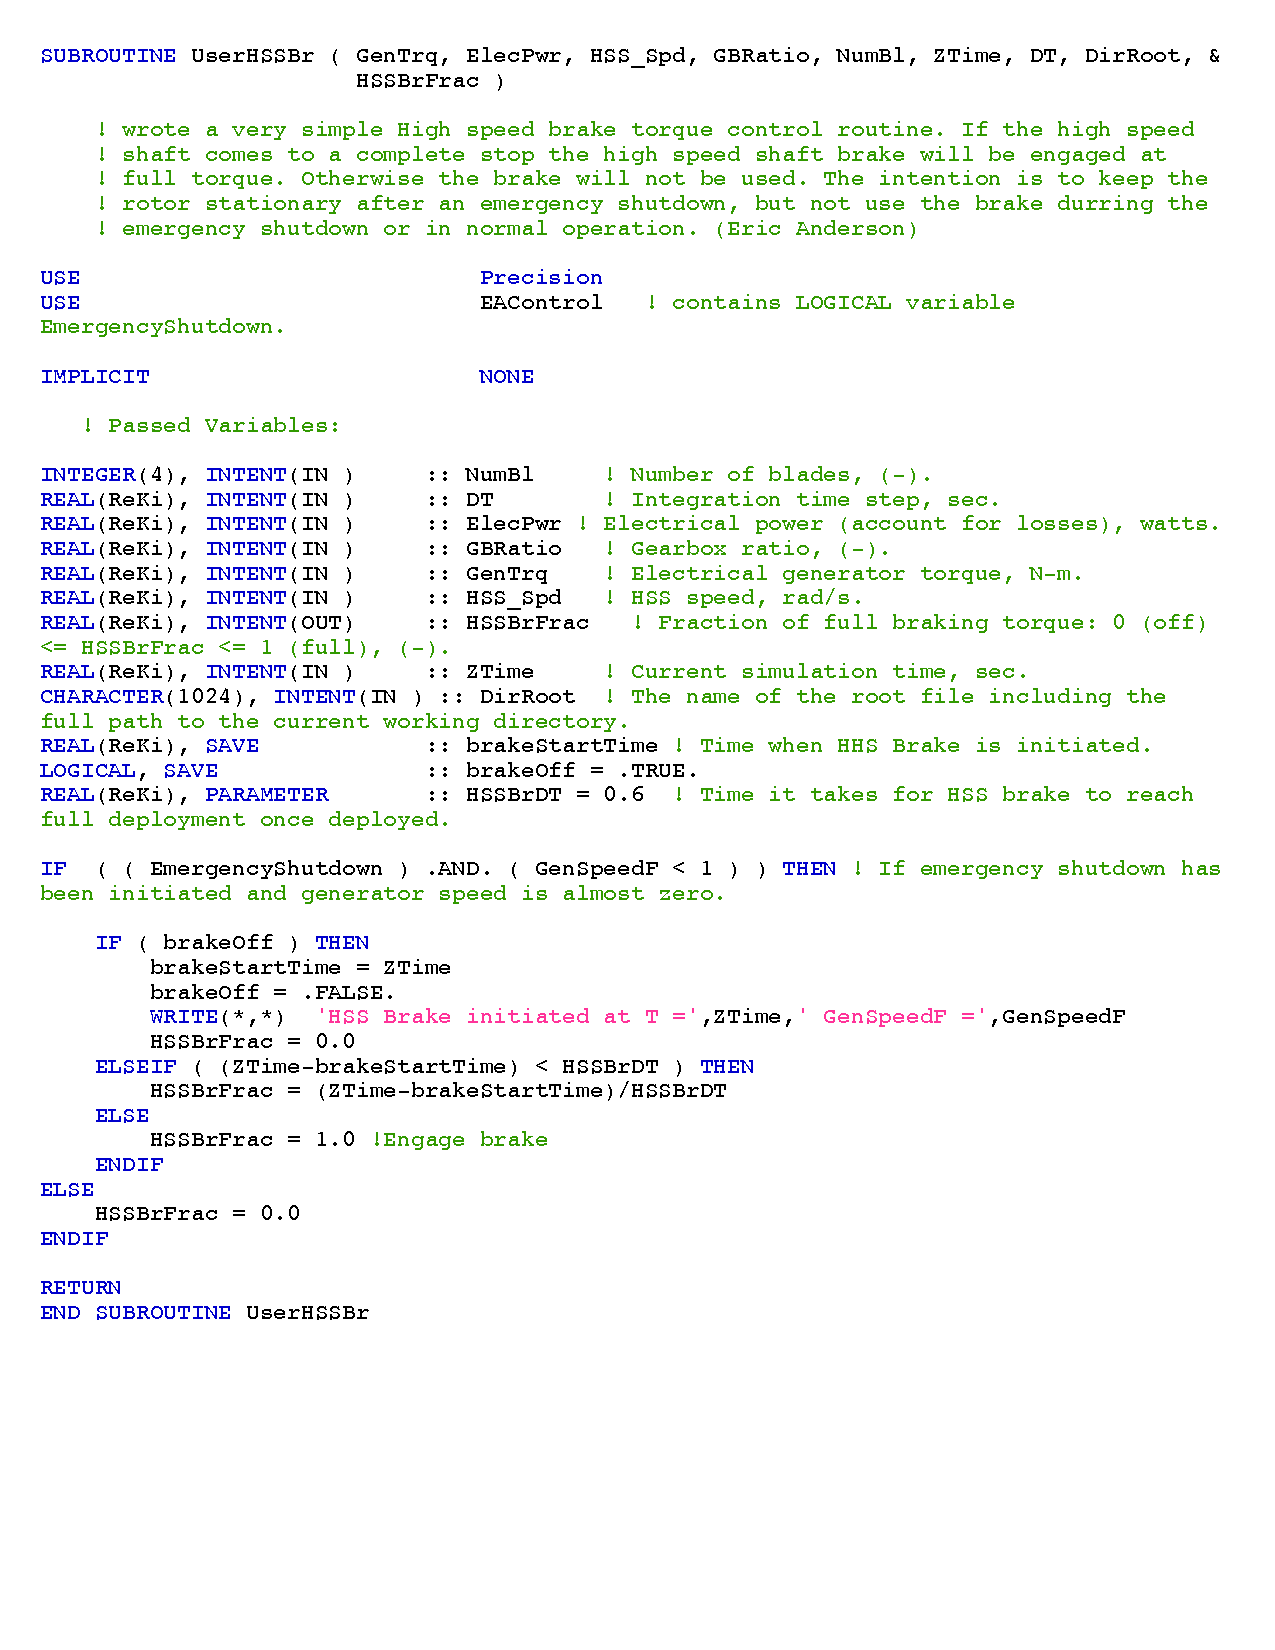
\includegraphics[width=\linewidth]{Figures/AppendixDFigures/figD-4.pdf}

%----------------------------------------------------------------------------------------
%	SECTION 5
%----------------------------------------------------------------------------------------
\section{Module EAControl()} \label{sectionD-5}
The following module is added to FAST\_Mods.f90.

\noindent
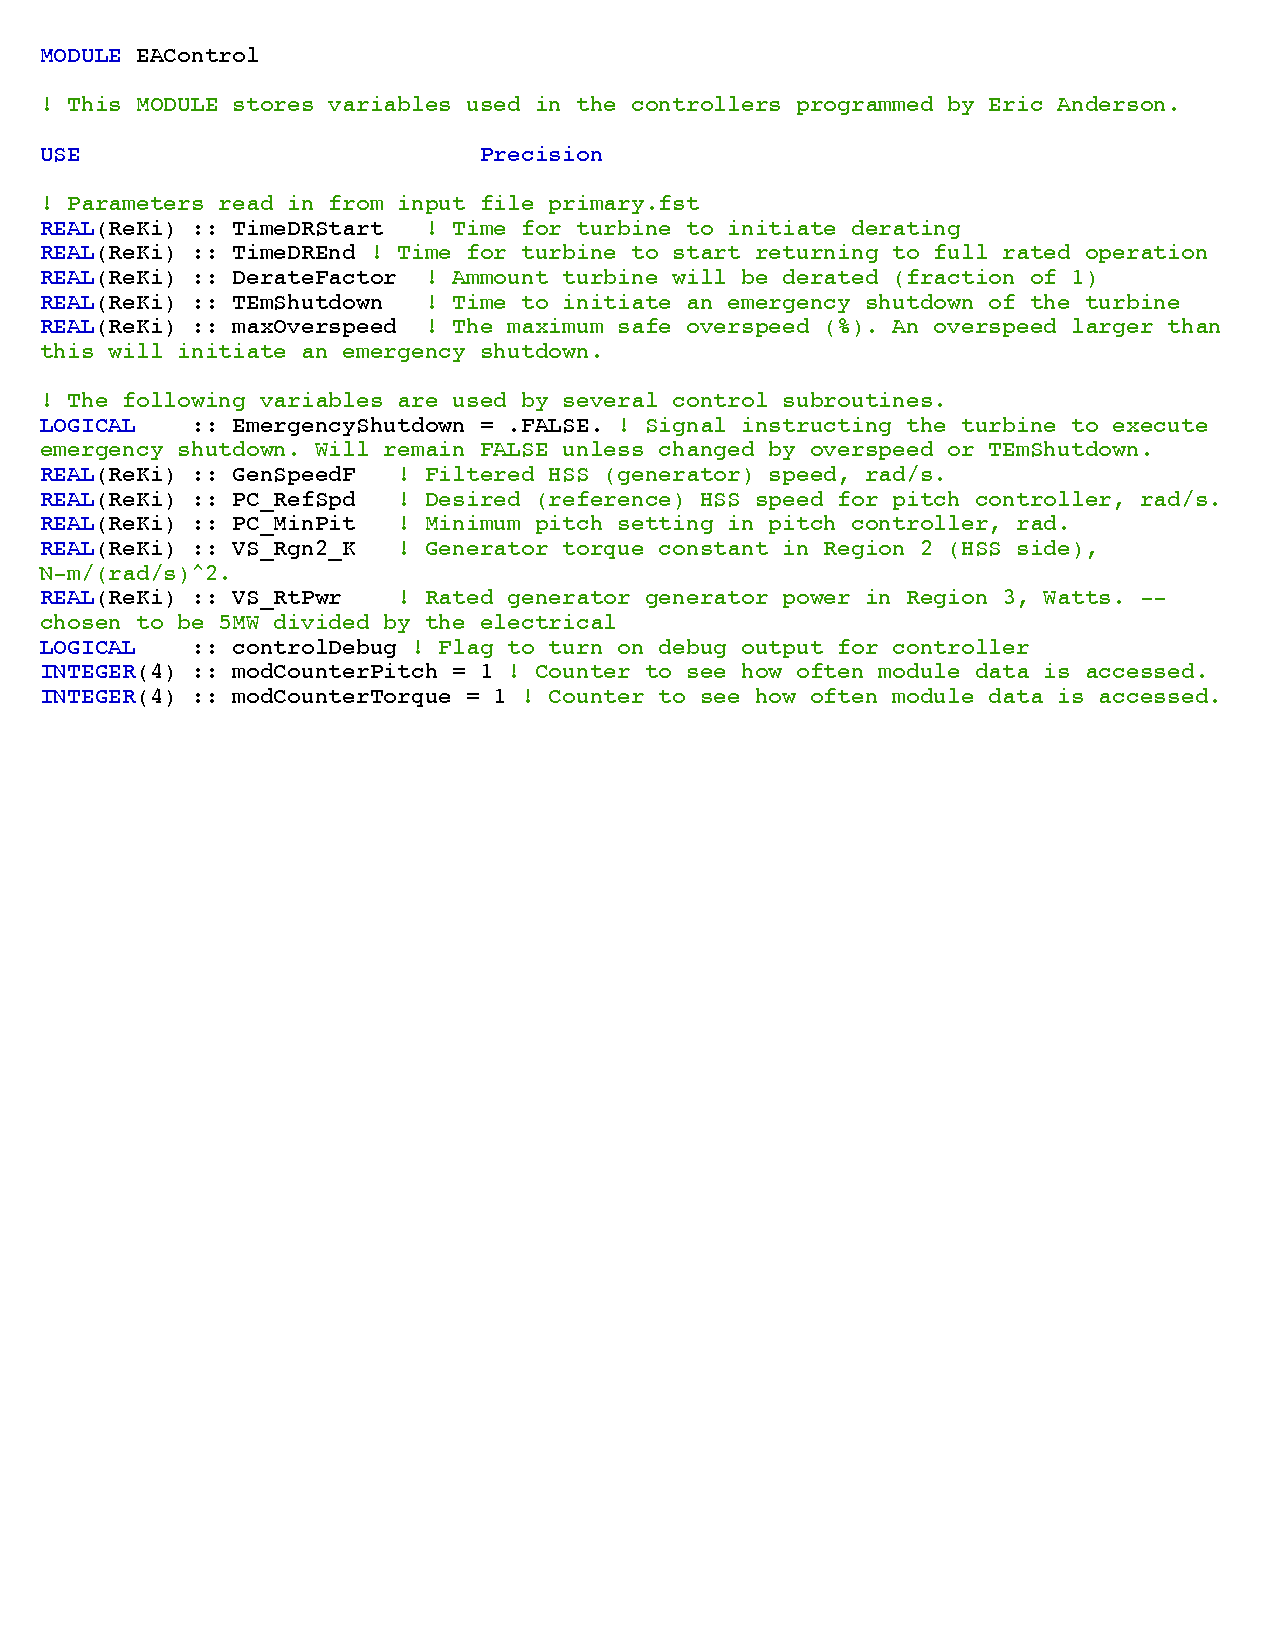
\includegraphics[width=\linewidth]{Figures/AppendixDFigures/figD-5.pdf}

%----------------------------------------------------------------------------------------
%	SECTION 7
%----------------------------------------------------------------------------------------
\section{Additions to input file primary.fst} \label{sectionD-7}

The following lines were added to the primary.fst input file just after the LINEARIZATION CONTROL section.

\noindent
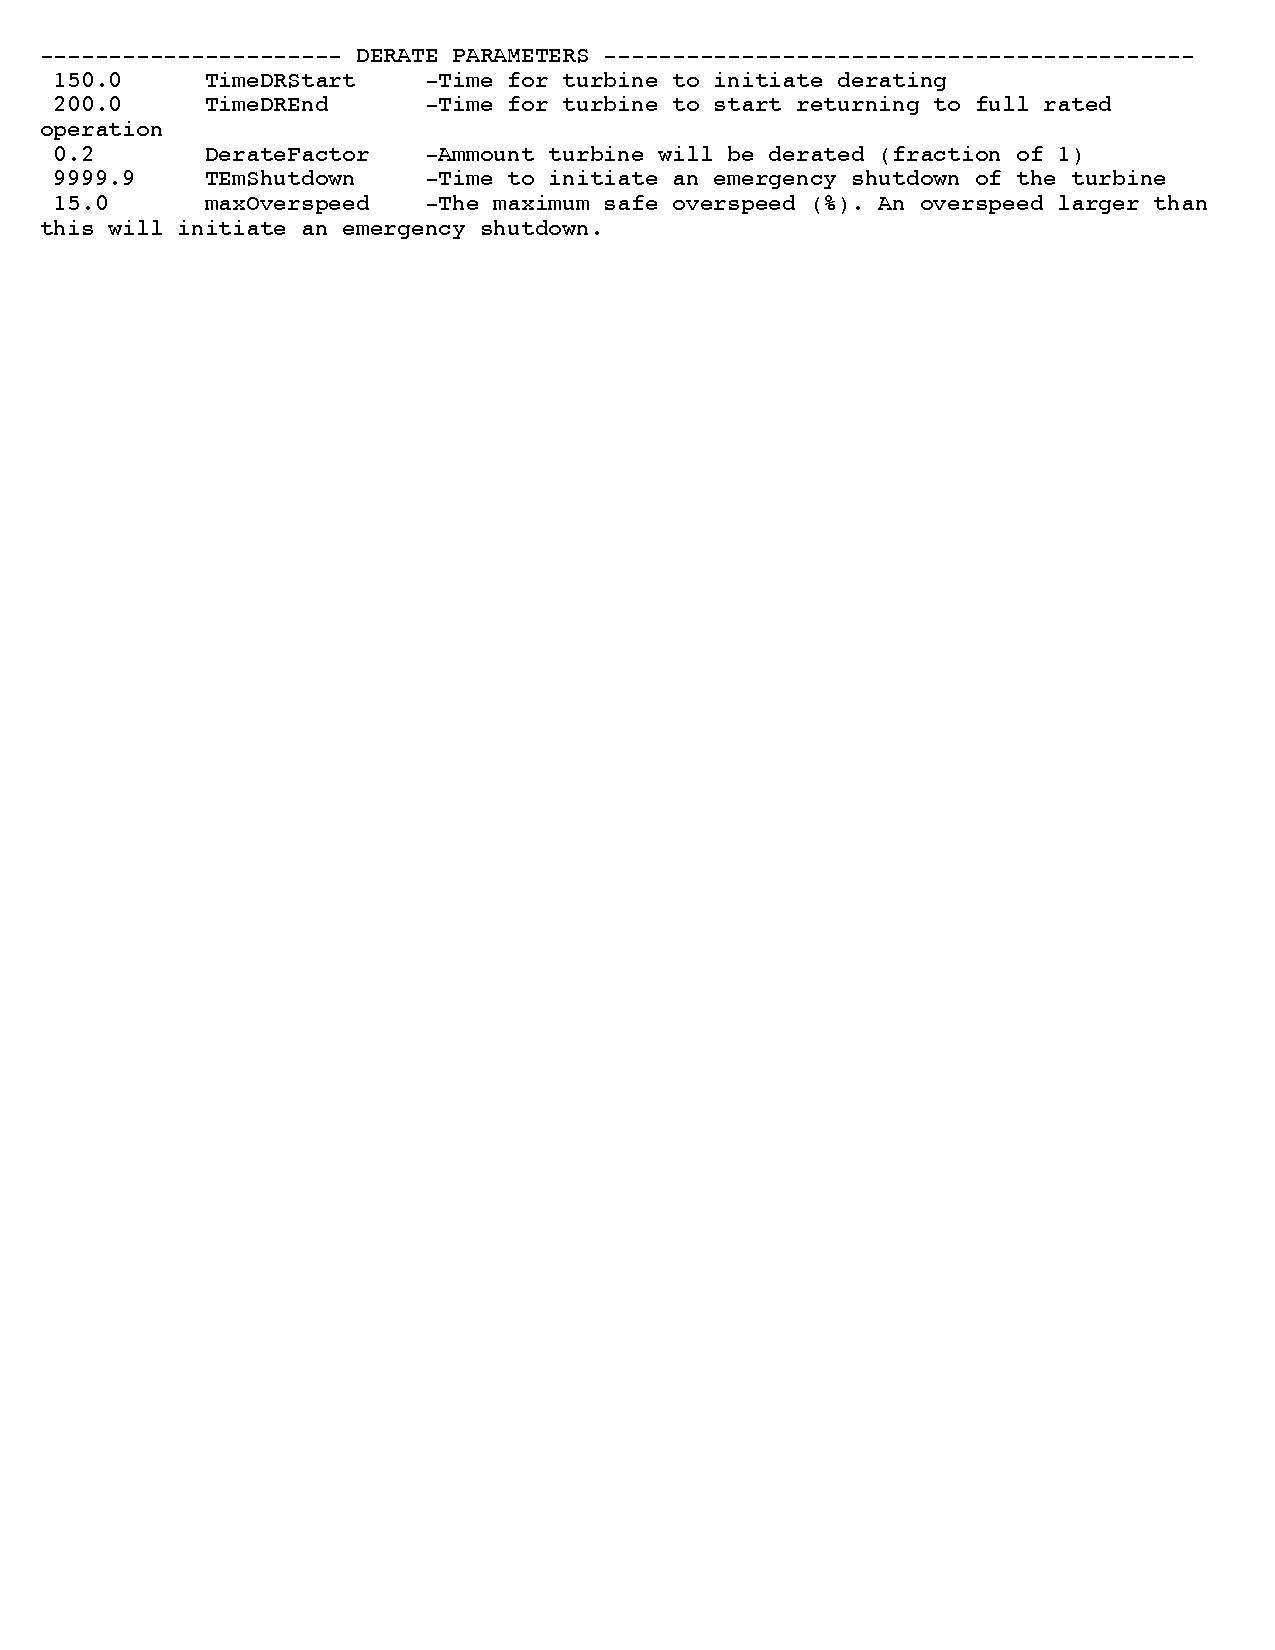
\includegraphics[width=.97\linewidth]{Figures/AppendixDFigures/figD-7.pdf}

%----------------------------------------------------------------------------------------
%	SECTION 6
%----------------------------------------------------------------------------------------
\section{Additions to FAST\_IO.f90} \label{sectionD-6}

The following lines are added to the FAST\_IO.f90 immediately after the FAST LINEARIZATION CONTROL PARAMETERS section.

\noindent
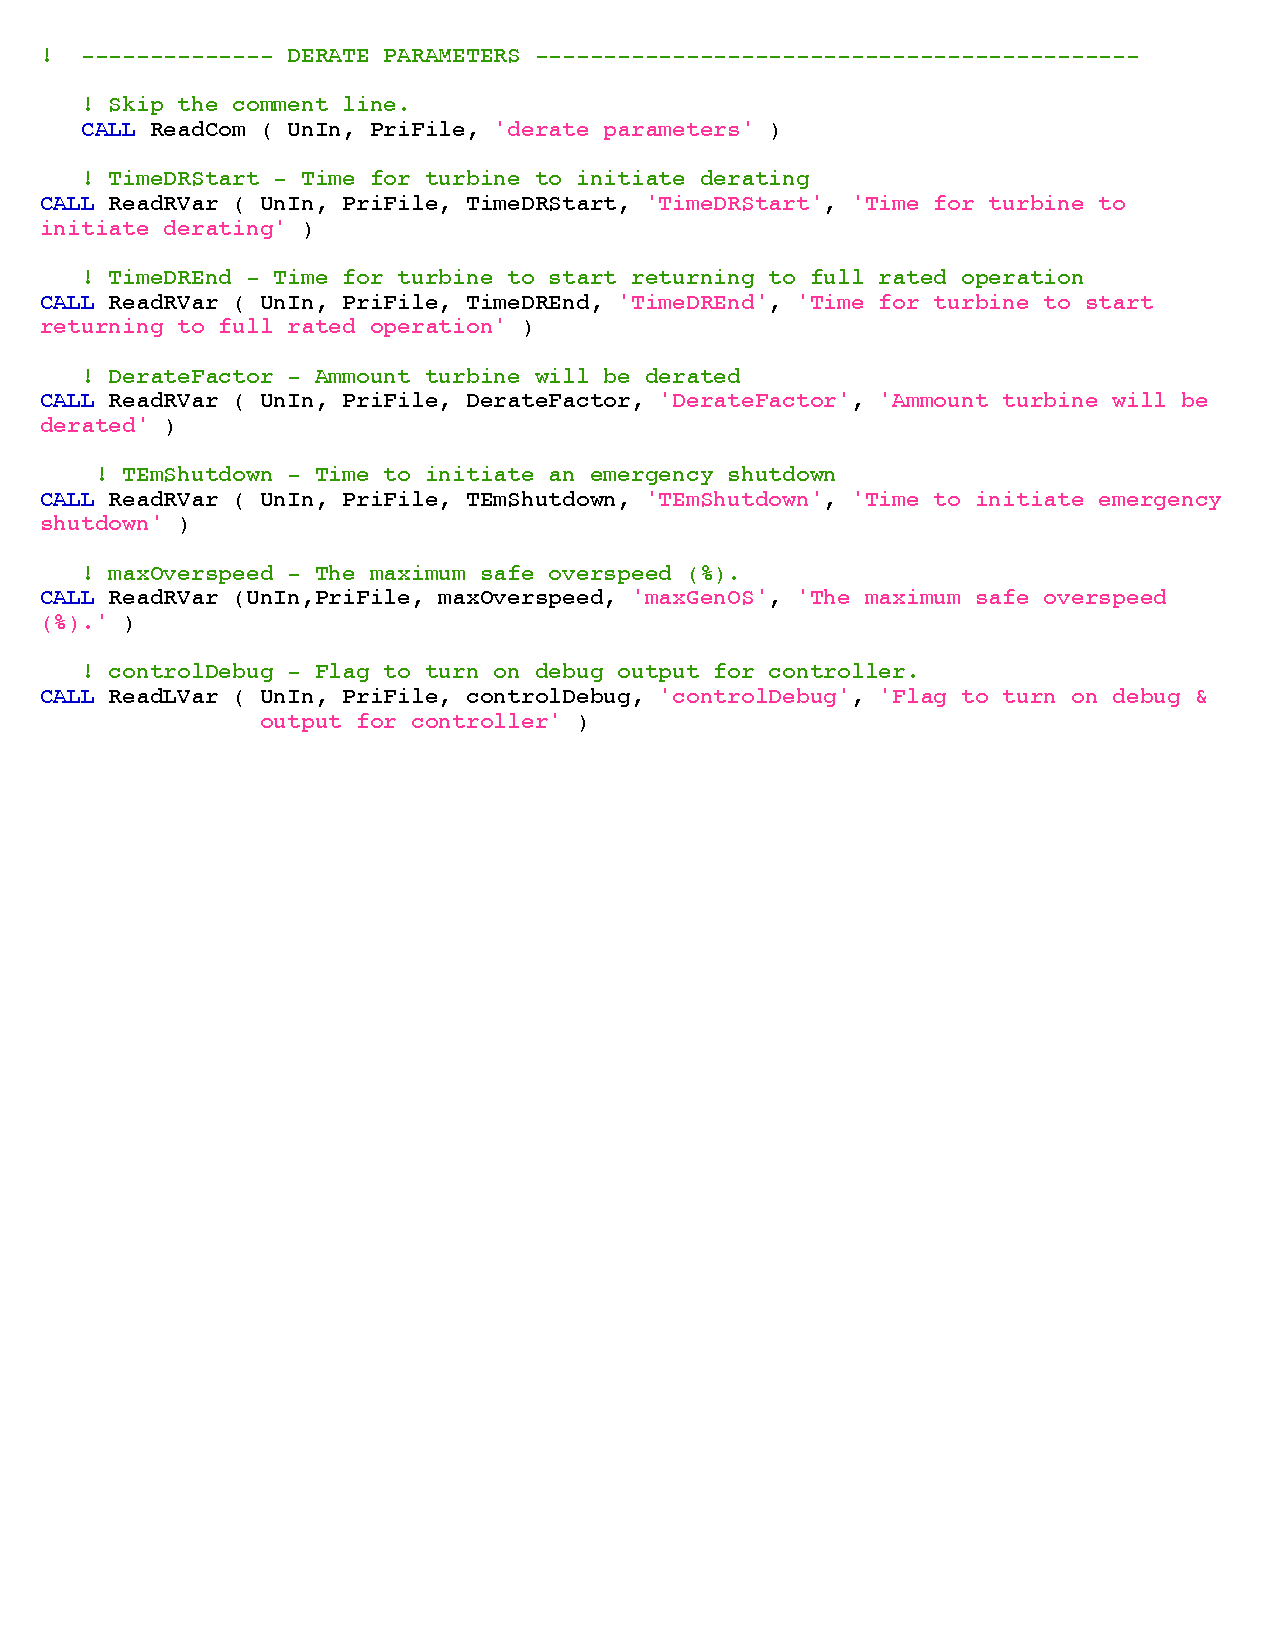
\includegraphics[width=\linewidth]{Figures/AppendixDFigures/figD-6.pdf}




